% Session 4 -- the ribbon spectrum: flat bulk Landau levels plus chiral edge
% branches, and why an impurity cannot backscatter an edge electron.
% Placement: sec. "Why an insulating bulk still conducts: edge states", after the
% ribbon / no-backscattering paragraph.
% Rendered by figures/blender/s04f01_ribbon.py, labels in figures/overlays/s04f01_ribbon.tex.
\begin{aqmfigure}{fig:s04:ribbon}{The quantum Hall ribbon. (a) The spectrum of a strip that is
infinite along $y$ and finite along $x$, computed for a width of $12\,\ell_B$ with hard walls. In
the bulk the Landau levels (4.6) are exactly flat, so they carry no current at all, but near each
boundary the guiding centre $x_0=\hbar k_y/B$ is pushed into the wall and the level bends up
strongly. These bending branches are the edge states, and each of them crosses the chemical
potential, the translucent plane, exactly once per edge, at the balls, so the number of chiral modes
at a given edge is equal to the number $N$ of filled Landau levels, here $N=2$. (b) The same
statement in real space, seen from above. The branches with $k_y>0$ have
$v_y=\hbar^{-1}\partial_{k_y}E>0$ and live on the right edge, and the branches with $k_y<0$ move in
the opposite direction and live on the left edge. To reverse the velocity of an electron we would
therefore have to move it to the other side of the sample, which no local impurity can do, and this
is why the edge transport has no dissipation.}
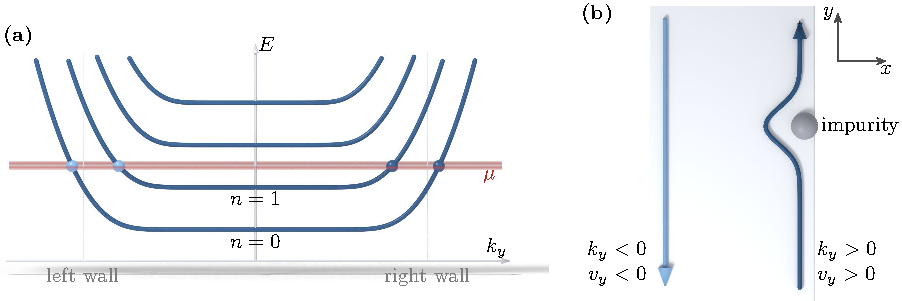
\includegraphics{figures/pdf/s04f01_ribbon.pdf}
\end{aqmfigure}
